\section{Grundlagen}
Dieses Kapitel erläutert die wesentlichen technologischen und konzeptionellen Grundlagen der entwickelten Lösung. Zunächst werden die eingesetzten Technologien vorgestellt, die eng mit dem bestehenden Technologie-Stack der Monidas-Plattform verknüpft sind. Anschliessend folgt die Erläuterung des Domänenmodells, das die konzeptionelle Basis für die Umsetzung bildet. Damit schafft dieses Kapitel die Voraussetzungen, um die technischen Entscheidungen und Implementierungen in den nachfolgenden Kapiteln nachvollziehen zu können.

\subsection{Technologien}
Für die Umsetzung des virtuellen Filesystems und des Language Servers werden Technologien eingesetzt, die gezielt auf die vorhandene Infrastruktur der Monidas-Plattform abgestimmt sind. Diese Technologien wurden in Abstimmung mit dem Auftraggeber ausgewählt, um Integration, Wartbarkeit und Erweiterbarkeit zu gewährleisten. Im Folgenden werden ausschliesslich jene Aspekte erläutert, die für das Verständnis und die Realisierung der in dieser Arbeit entwickelten Lösung relevant sind.

%Zum Einsatz kommen dabei die Graphdatenbank Selva und das JavaScript-Framework Based, welche nachfolgend näher erläutert werden.

\subsubsection*{Selva}
Als Datenbanktechnologie kommt die Graphdatenbank \textit{Selva}\footnote{\url{https://github.com/atelier-saulx/selva}} zum Einsatz. 


\paragraph{Datenbankschema}
Selva definiert das Datenmodell mithilfe eines Schemas, welches Objekttypen, deren Felder sowie erlaubte Datentypen beschreibt. Unterstützt werden einfachen Datentypen wie \texttt{string}, \texttt{int} und \texttt{boolean} sowie komplexere Beziehungstypen wie \texttt{reference} (für 0:1-Beziehungen) und \texttt{references} (für 0:n-Beziehungen).

Auf Datentyp-Ebene führt Selva grundlegende Validierungen automatisch durch. Beispielsweise prüft Selva, ob die Werte eines String-Feldes tatsächlich Zeichenketten sind oder ob Felder vom Typ \texttt{email} ein gültiges E-Mail-Format besitzen.

Weitergehende Anforderungen, wie Pflichtfelder, Pfadeinschränkungen, bidirektionale Verknüpfungen oder Einschränkungen bei der Erstellung neuer Objekte, werden von Selva nicht standardmässig unterstützt. Diese Constraints sind jedoch notwendig, um eine konsistente und fehlerfreie Verwaltung komplexer Datenstrukturen sicherzustellen. Deshalb wurden diese im Rahmen dieser Arbeit eigenständig definiert und implementiert. Eine detaillierte Erläuterung hierzu erfolgt in Abschnitt \ref{Constraints}.


Ein vereinfachtes Schema zur Verdeutlichung könnte wie folgt aussehen:


Im gezeigten Beispiel werden drei Objekttypen definiert: \texttt{Sensor}, \texttt{Location} und \texttt{Threshold}. Neben einfachen Attributen wie Name oder geografischen Angaben umfasst das Schema auch komplexe Beziehungsfelder. So besitzt der Sensor eine eindeutige Standortzuweisung sowie mehrere Grenzwerte.

\paragraph{Query Domain Specific Language (DSL)}
Für Abfragen und Datenmanipulationen bietet Selva eine eigene Query DSL, die auf JavaScript-Objekten basiert. Diese DSL definiert, welche Daten abgefragt und wie diese präsentiert werden sollen. Dabei unterscheidet Selva zwischen:

\begin{itemize} \item \textbf{Felder}, welche gespeicherte Eigenschaften repräsentieren und einfache sowie komplexe, verknüpfte Daten umfassen.
\item \textbf{Operatoren}, welche bestimmen, wie die Daten sortiert oder gefiltert werden. Dazu gehört auch der Operator \textbf{alias}, mit dem Objekte direkt über ihren Alias statt über ihre interne ID abgefragt werden können.
\end{itemize}

Im Anhang \ref{sec:selva-operationen} befinden sich konkrete Beispiele zur Nutzung der Query DSL, darunter auch die Verwendung eines Alias.

\paragraph{Selva-API}
Zur Interaktion zwischen Anwendung und Datenbank bietet Selva eine eigene API, welche grundlegende Operationen zur Datenmanipulation und -abfrage bereitstellt. Dazu gehören das Abfragen von Daten (\texttt{get}), das Erstellen und Aktualisieren von Objekten (\texttt{set}), das Löschen von Daten (\texttt{delete}) sowie das Beobachten von Datenänderungen in Echtzeit (\texttt{observe}). Weitere Funktionen der API ermöglichen das Abfragen (\texttt{getSchema}) und Anpassen (\texttt{updateSchema}) des Datenbankschemas, das Erzeugen eindeutiger IDs (\texttt{id}) sowie die Bestimmung des Objekttyps auf Basis einer ID (\texttt{getTypeFromId}).

Die praktische Verwendung aller genannten Operationen wird im Anhang \ref{sec:based-operationen} anhand konkreter Code-Beispiele gezeigt. Diese Operationen wurden für die Implementierung der im Rahmen dieser Arbeit entwickelten Funktionalitäten eingesetzt.

\subsubsection*{Based}
tbd
https://github.com/atelier-saulx/based/blob/v3/packages/client/docs/get-started.md
%Zur weiteren Abstraktion der Datenbankkommunikation kommt ergänzend zu Selva das JavaScript Framework Based\footnote{\url{https://github.com/atelier-saulx/based}} zum Einsatz. Dieses stammt vom selben Entwicklungsteam wie Selva und ist somit gezielt auf deren Integration ausgelegt.

%Based stellt dazu zwei verschiedene Operationsarten bereit:
%\begin{itemize} 
%\item \textbf{Queries} ermöglichen den lesenden Zugriff auf Daten und unterstützen neben einmaligen Abfragen auch  Subscriptions.

%\item \textbf{Functions} hingegen führen schreibende Operationen aus, beispielsweise das Erstellen, Aktualisieren oder Löschen von Daten. 

%Zusätzlich können Functions serverseitige Logik enthalten. Dadurch lassen sich Validierungen, Prüfungen oder komplexere Abläufe direkt auf dem Server umsetzen, bevor Daten gespeichert werden.
%\end{itemize}

%Die konkrete Anwendung von Based wird ebenfalls anhand praxisnaher Beispiele im Anhang \ref{sec:selva-operationen} dargestellt.

\subsubsection*{VS Code}
VS Code dient als Plattform für zwei getrennte Extensions. Für das virtuelle Filesystem kommt die \textit{FileSystemProvider}-API\footnote{\url{https://code.visualstudio.com/api/references/vscode-api\#FileSystemProvider}} zum Einsatz. Die API stellt Funktionen bereit, um ein eigenes Filesystem mit Dateien und Ordnern über URI-Pfade zu verwalten. Dazu gehören das Erstellen, Löschen und Lesen von Inhalten. 

Für die Editorunterstützung wird das Language Server Protocol verwendet. Die Integration erfolgt nach den Vorgaben des offiziellen \textit{Language Server Extension Guide}\footnote{\url{https://code.visualstudio.com/api/language-extensions/language-server-extension-guide}}.

tbd wird inhaltlich noch angepasst

\subsubsection*{Node.js / TypeScript}
tbd

\pagebreak

\subsection{Domänenmodell}
Zur einheitlichen Darstellung und besseren Verständlichkeit der entwickelten Lösung wurde für diese Arbeit ein Domänenmodell aus dem Bereich E-Commerce definiert. Dieses Modell bildet ein beispielhaftes Szenario ab, das für die nachfolgenden Kapitel als Referenz dient. Die entwickelte Lösung ist jedoch nicht auf dieses spezielle Modell beschränkt, sondern kann auf beliebige andere Domänenmodelle übertragen werden, ohne dass Änderungen an der Kernfunktionalität nötig sind. Im diesem Abschnitt wird das erstellte Domänenmodell basierend auf der UML-Darstellung in Abbildung~\ref{fig:uml_modell} erläutert.

\begin{figure}[H]
  \centering
  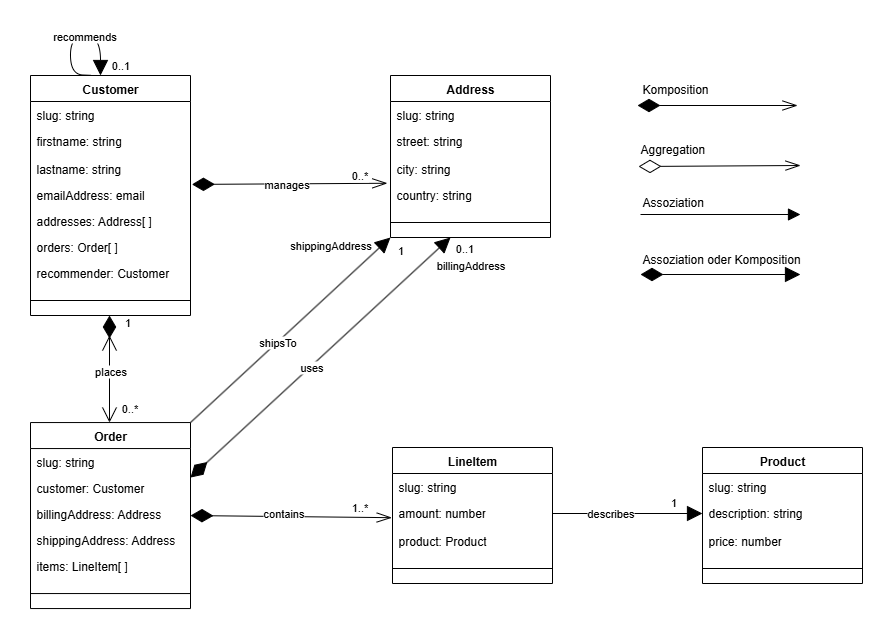
\includegraphics[width=\linewidth]{UML.png}
  \caption{UML-Darstellung des für diese Arbeit definierten Domänenmodells.}
  \label{fig:uml_modell}
\end{figure}

Das definierte Domänenmodell besteht aus den Entitäten \texttt{Customer}, \texttt{Order}, \texttt{Address}, \texttt{Product} und \texttt{LineItem}. Zur eindeutigen Identifikation im virtuellen Filesystem verfügt jede Entität zwingend über das Attribut \texttt{slug}. Der \texttt{slug} ist ein menschenlesbarer Bezeichner, der zur Generierung eindeutiger URI-Pfade verwendet wird. Wird beispielsweise ein Kunde mit dem \texttt{slug} „max“ erstellt, entsteht daraus der eindeutige URI-Pfad \texttt{/Customers/max}. Die konkrete Bedeutung und Nutzung des Attributs \texttt{slug} im Kontext des virtuellen Filesystems wird in Abschnitt~\ref{vfs-umsetzung} detailliert beschrieben.

tbd Beschreibung des UML